
\section{Betriebsszenarien}
\label{s:Betriebsszenarien}
Betriebsszenarien helfen die vorher beschriebene Betrieb- und Infrastrukturkosten in Anwendung zu bringen 
und eine mögliche Entwicklung in der nahen Zukunft zu zeigen. 
Die Größe des Flughafens beeinflusst die Infrastrukturkosten. 
Bei einem größeren Flughafen werden die Betriebsdifferenzen deutlicher, da das Verkehrsaufkommen wesentlich höher ist.
Größere Flughäfen abfertigen täglich mehr Flugzeuge als Regionalflughäfen, 
was dazu führt, dass mehr Abfertigungsplätze umgerüstet/versorgt werden müssen und mehr Arbeitskräfte geschult werden müssen.

Deshalb wird für die Betriebsszenarien der Flughafen Frankfurt gewählt, der fungiert als bedeutendes Luftverkehrsdrehkreuz
und zudem der größte Verkehrsflughafen Deutschlands.
Der Fraport meldete im Jahr 2023 insgesamt 423764 gewerbliche Flugbewegungen, was im Durchschnitt 1160 Flugbewegungen pro Tag ausmacht. 
Es wird angenommen, dass die Hälfte davon Abflüge sind, also müssen 580 Flugzeuge am Tag abgefertigt werden.
%
Die Gesamtbewegungen teilen sich nach Entfernungen folgend auf \cite{fraport2023frankfurt}:
\begin{itemize}
    \item Kurzstrecken (bis 2500 km) sind bei 72,8 \%;
    \item Mittelstrecken (bis 6000 km) sind 9,3 \%;
    \item Langstrecken (ab 6000 km) die restlichen 17,9 \%. 
    \end{itemize}
Da ist nicht explizit definiert wird, welche Entfernungen Flugzeuge zurücklegen, werden die Betriebskosten anhand vorher beschriebene Distanzen berechnet.
Dabei wird für Kurzstrecken eine Entfernung von 400 km genommen und für Langstrecken eine Distanz von 6000 km.
Für Mittelstrecken wird die gleichen Werte wie bei Langstreckenflügen verwendet, jedoch mit einer anderen Distanz von 4000 Kilometer,
dass Treibstoffverbrauch pro Stunde sich nicht ändern wird.

Anhand dessen wird eine Flotte mit 580 Flugzeugen aufgestellt, wo die alternativen Antriebe im Einsatz sind.
Aufgrund der Flugeinschränkungen in der Nacht wird es angenommen, dass die Flüge von 6 bis 24 Uhr gleichmäßig stattfinden. 
Wie bereits diskutiert wurde, können Kurzstrecken-Flüge durch den Einsatz von batteriebetriebenen Flugzeugen ersetzt werden. Hier wird
auch als Ersatz SAF mitberechnet. Es ist nennenswert, dass nur Teil der tatsächlichen Nachfrage des Kurzstrecken-Bedarfs 
dadurch gedeckt werden kann. Die Mittel- und Langstrecken werden durch Flugzeuge mit Wasserstoffturbine und SAF versorgt/erfüllt.
%
In Betrachtung des tatsächlichen Flugplans sind die Spitzenstunden im Laufe des Tages zu finden, wo
der Verkehrsfluss stärker als im Durschschnitt ist. In diesem Fall werden höhere Infrastruktur- und Betriebskosten zu erwarten.
Indessen um die Interpretation zu erleichtern, wird in dieser Arbeit angenommen, dass stündlich die gleiche Anzahl an Flugzeugen 
am Flughafen abgewickelt werden. 
%
Die Aufteilung den Antrieben für jedes Szenario ist in der Abbildung \ref{betriebsszenarien} dargestellt.
%
\begin{figure}[h]
	\centering
	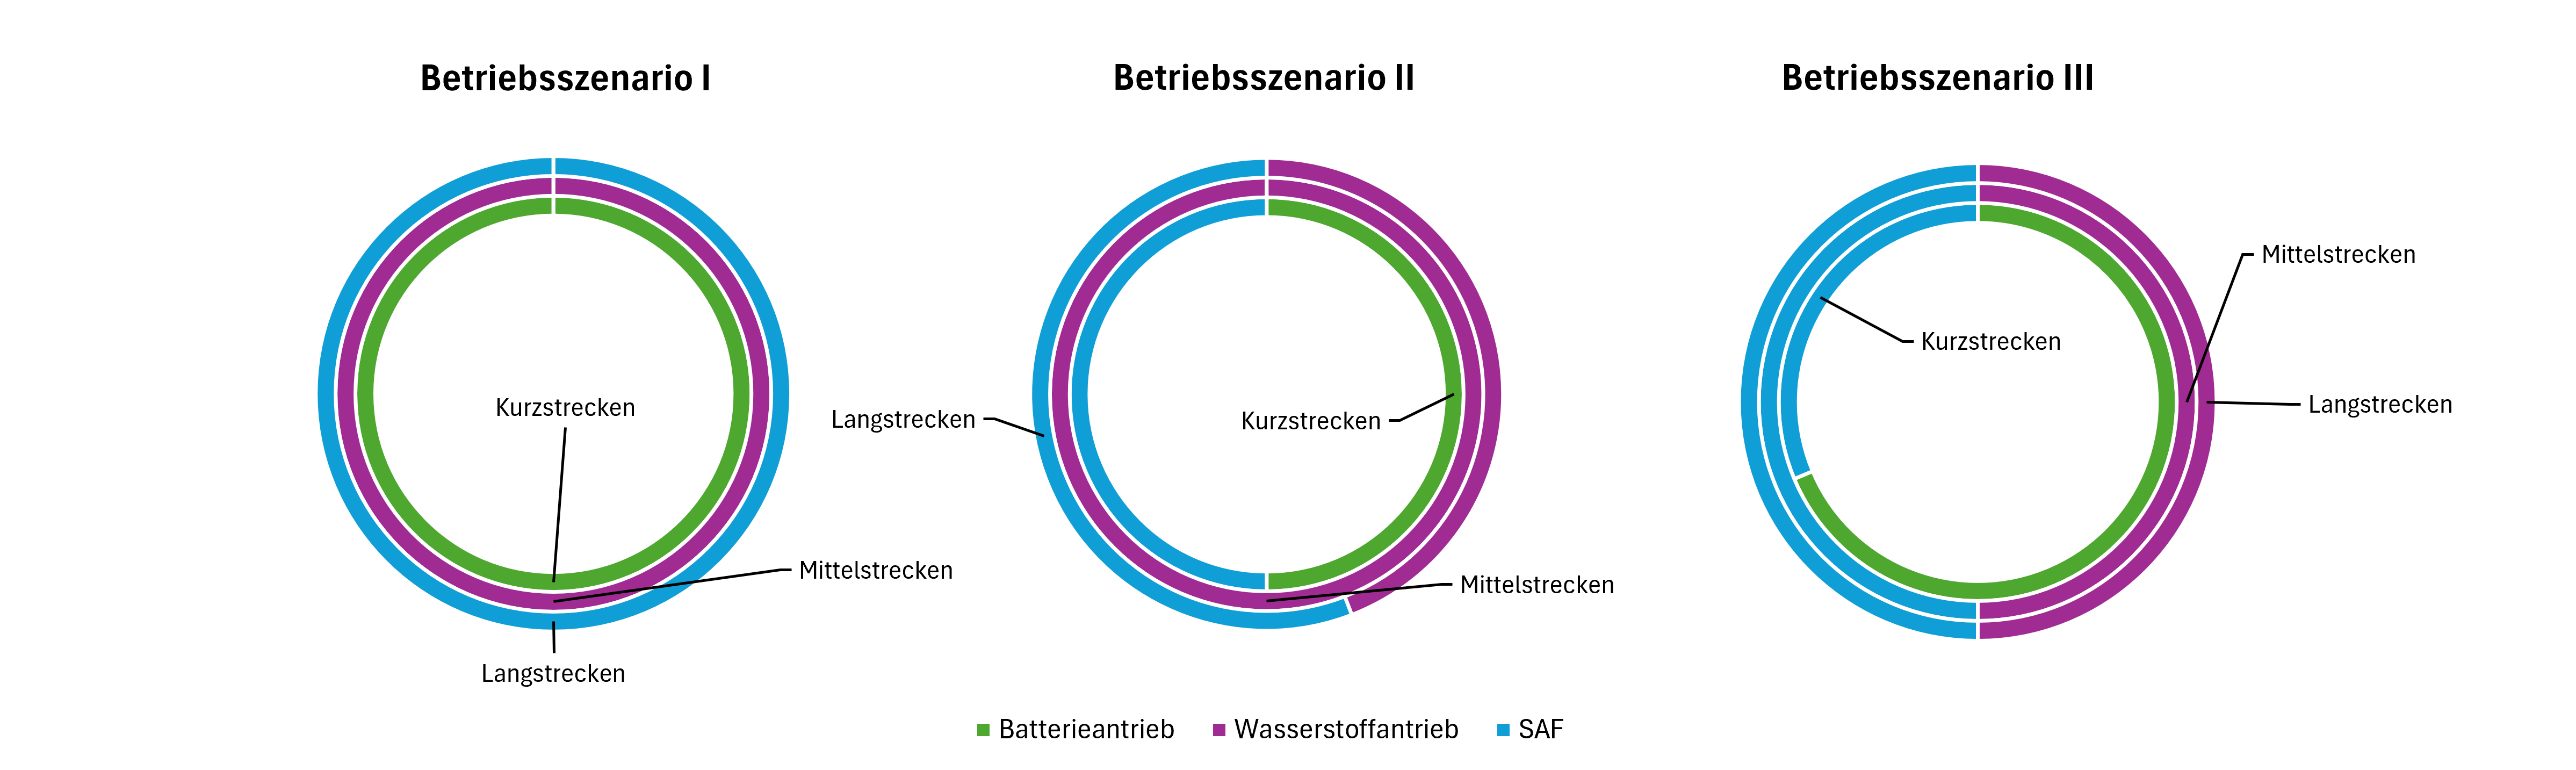
\includegraphics[width=1.0\linewidth]{Bilder/Betriebsszenarien.png}
	\caption[Betriebsszenarien]{Aufteilung der Flugzeugflotte nach Antriebsart}
	\label{betriebsszenarien}
\end{figure}
%
In dem \textbf{ersten Betriebsszenario} wird angenommen, dass:
\begin{itemize}
    \item Die Kurzstrecken durch die BA komplett ersetzt werden;
    \item Die Mittelstrecken werden vollkommen durch WA;
    \item und die Langstrecken durch die SAF bedient.
\end{itemize}
Das \textbf{zweite Betriebsszenario} wird mit folgender Aufteilung berechnet:
\begin{itemize}
    \item Die Hälfte der Kurzstrecken wird durch BA versorgt und die andere Hälfte durch SAF; 
    \item die Mittelstrecken werden genauso, wie im ersten Szenario komplett durch die Wasserstoffflugzeuge bedient und 
    \item Langstrecken sind 10 \% der Gesamtflotte durch den SAF und den restlichen Anteil Wasserstoff.
\end{itemize}
Das \textbf{dritte Szenario}:
\begin{itemize}
    \item 50 \% der Kurzstrecken sind von Batterie-Antrieb, die restlichen 22,8 \% sind mit SAF betrieben
    \item Mittelstrecken: die Hälfte der Mittelstrecken sind mit WA und die andere Hälfte mit SAF
    \item Langstrecken: die Hälfte der Mittelstrecken sind mit WA und die andere Hälfte mit SAF
\end{itemize}
%
Daraus ergibt sich die folgende Flottenaufteilung für die einzelnen Szenarien:
\begin{table}[h]
	\begin{center}
    \caption{Werte und Annahmen der BA-Infrastruktur}
	\label{BA_Infrastrukturtab}
	\begin{tabular}{|c|c|c|>{\centering\arraybackslash}p{3cm}|c|}
		\hline
		\multicolumn{4}{|c|}{\textbf{Szenario I}} \\ \hline
		 & \textbf{Batterieantrieb} & \textbf{Wasserstoffantrieb} & \textbf{SAF} \\ \hline
		Kurzstrecken & 422 & - &-\\ \hline
      	Mittelstrecken & -  & 54 &- \\ \hline
		Langstrecken & - & - &104 \\ \hline
		\multicolumn{4}{|c|}{\textbf{Szenario II}} \\ \hline
		Kurzstrecken & 211 &- &211\\ \hline
      	Mittelstrecken &  - & 54 &- \\ \hline
		Langstrecken &- & 46  &58 \\ \hline
		\multicolumn{4}{|c|}{\textbf{Szenario III}} \\ \hline
		Kurzstrecken & 290 &- &132\\ \hline
      	Mittelstrecken &  - & 27 & 27 \\ \hline
		Langstrecken &  -& 52 &52 \\ \hline
	\end{tabular}
    \end{center}
\end{table}